\documentclass[tikz,border=4pt]{standalone}
% Shared setup for the foundation-model diagrams, in the AFRICAST palette
\usepackage{fontspec}
\usepackage[sfdefault]{FiraSans}
\usepackage{amsmath}
\usepackage{unicode-math}
\setmathfont{Fira Math}
\usetikzlibrary{arrows.meta}
\definecolor{ink}{HTML}{1F2A36}
\definecolor{MonashBlue}{HTML}{3B75AC}
\definecolor{Orange}{HTML}{B5570F}
\color{ink}
\tikzset{every picture/.style={draw=ink,>=stealth}}
\hyphenpenalty=10000
\exhyphenpenalty=10000

\begin{document}
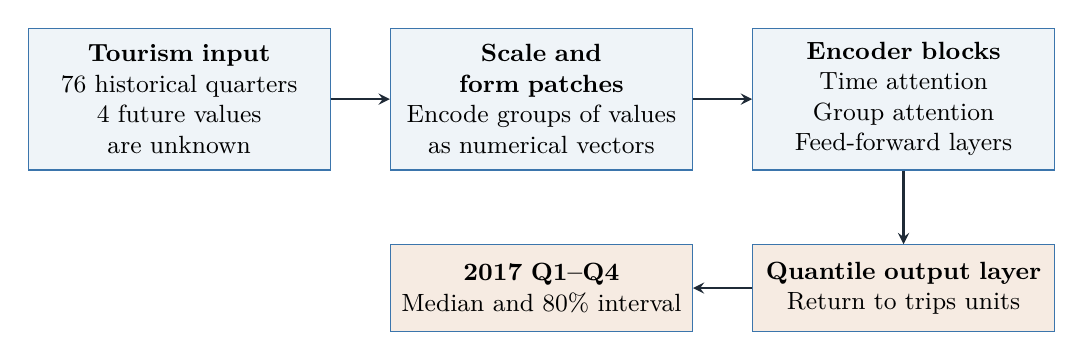
\begin{tikzpicture}[>=stealth,every node/.style={font=\fontsize{9}{11}\selectfont,align=center},
box/.style={draw=MonashBlue,fill=MonashBlue!8,text width=3.6cm,minimum height=1.8cm}]
\node[box] (data) at (0,0) {\textbf{Tourism input}\\76 historical quarters\\4 future values\\are unknown};
\node[box] (embed) at (4.6,0) {\textbf{Scale and form patches}\\Encode groups of values\\as numerical vectors};
\node[box] (encoder) at (9.2,0) {\textbf{Encoder blocks}\\Time attention\\Group attention\\Feed-forward layers};
\node[box,fill=Orange!12,minimum height=1.1cm] (head) at (9.2,-2.4) {\textbf{Quantile output layer}\\Return to trips units};
\node[box,fill=Orange!12,minimum height=1.1cm] (forecast) at (4.6,-2.4) {\textbf{2017 Q1--Q4}\\Median and 80\% interval};
\draw[->,thick](data)--(embed);\draw[->,thick](embed)--(encoder);
\draw[->,thick](encoder)--(head);\draw[->,thick](head)--(forecast);
\end{tikzpicture}
\end{document}
